\documentclass[russian]{article}
\usepackage[T1]{fontenc}
\usepackage[utf8]{inputenc}
\usepackage{geometry}
\geometry{verbose,tmargin=2cm,bmargin=2cm,lmargin=1cm,rmargin=1cm}
\usepackage{float}
\usepackage{textcomp}
\usepackage{amssymb}
\usepackage{graphicx}
\usepackage{babel}
\usepackage[T2A]{fontenc}

\makeatletter
\@ifundefined{date}{}{\date{}}


\begin{document}

\title{Матлогика. HW\#5}
\author{Тураев Тимур, 504 (SE)}

\maketitle

\paragraph{1} \textit{Доказать, что существует $k\in \mathbb{N}$, такое что неразрешимо множество \[ H^k = \{ x | \langle k \rangle (x) \neq \bot \} \]}

На самом деле не очень понятно как решать. Примеры из лекции и из практики мне ясны, а вот как приложить их к этому примеру, я не знаю…

\paragraph{2} \textit{Сигнатура $(f^1, =^2)$, носитель $\mathbb{Z}$, нормальная интерпретация, $[f](x) = x + 2$. Невыразимый предикат $y = x + 1$. Найдите автоморфизм, относительно которого данный предикат неустойчив.}

Предлагается такой автоморфизм: если $x$ четное, то $x \rightarrow x +2$, иначе $x \rightarrow x$. Или короче (но запутаннее): $x \rightarrow x + 2 - (x \bmod 2) * 2$. То есть ко всем четным прибавить 2. Это действительно автоморфизм (проверить легко).
Предикат $y = x + 1$, ясно, неустойчив: слева и справа числа разной четности и прибавление числа $2$ приведет к неверной формуле.

\paragraph{3} \textit{Сигнатура $(=^2, P^2)$, носитель $\mathbb{N}_+$, нормальная интерпретация, $[P](x, y) = x | y$. Невыразимый предикат $x = 2$. Найдите автоморфизм, относительно которого данный предикат неустойчив.}

Предлагается такой автоморфизм: разложим $x$ на простые множители. Затем, заменим все двойки в этом разложении на тройки, а все тройки -- на двойки. (формально для числа $1$ нет разложения на простые, то просто дополним по определению $1 \rightarrow 1$) Более формально $x = 2^a \cdot 3^b \cdot k \rightarrow 2^b \cdot 3^a \cdot k$, где $2 \nmid k \wedge 3 \nmid k$
Предикат $x = 2$, ясно, неустойчив, так как $2 \to 3$

\paragraph{4} \textit{Построить дерево вывода.
\[
\vdash \exists y \forall x Q(x,y) \rightarrow \exists x Q(x, x)
\]}

\begin{center}
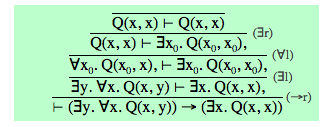
\includegraphics[scale=0.64]{4.png} 
\end{center}

\paragraph{5} \textit{Построить дерево вывода.
\[
\vdash \exists x (P(y) \vee P(f(z)) \rightarrow P(x))
\]}

\begin{center}
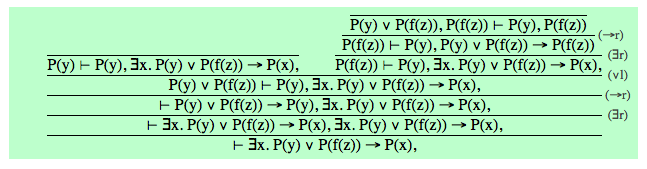
\includegraphics[scale=0.64]{5.png} 
\end{center}

\paragraph{6} \textit{Построить дерево вывода.
\[
\vdash \exists x \forall y (P(x) \rightarrow P(y))
\]}

\begin{center}
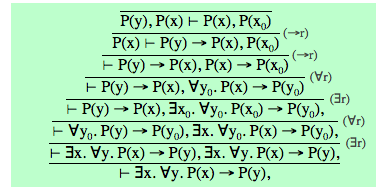
\includegraphics[scale=0.64]{6.png} 
\end{center}

\end{document}
